\chapter{Sprint 3: Container management}
In this chapter, we focus on Sprint 3, dedicated to container management.
This sprint aims to develop functionalities for handling container images,
including fetching images, instantiating containers, and managing clusters.
By leveraging containerization, we streamline application deployment, improve scalability, and enhance orchestration.
We will explore detailed processes in container management to ensure efficient and reliable operations.
Additionally, we will include sequence diagrams to illustrate key processes such as instantiating containers, and creating clusters, providing a clear understanding of interactions and workflows.


\pagebreak

\section{Analysis of Sprint 3 Requirements}
In this section, we will analyze the requirements for Sprint 3, which focuses on container management. This sprint involves developing and implementing functionalities related to container images, including fetching images, instantiating containers, and managing container clusters. 

\subsection{Use cases diagram of Sprint 3}

The following figure (\hyperref[fig:sprint_use_cases]{Figure \ref{fig:sprint_use_cases-manage_users2}})  represents the uses cases of our sprint.
\begin{figure}[h]
  \center
%\hspace*{-0.9in}
  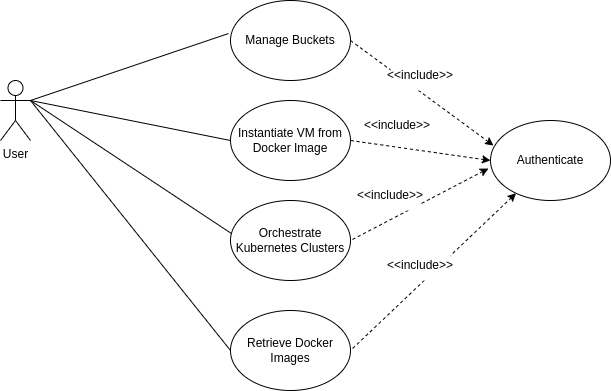
\includegraphics[width=10cm]{./chapters/sprint3/sprint_use_cases.png}
  \caption{Sprint use cases diagram}
  \label{fig:sprint_use_cases}
\end{figure}

The use case diagram for container management illustrates the interactions between users and the system for managing container images and clusters. The primary use cases include:

\begin{itemize}
  \item \textbf{Fetch Image:} Users can retrieve container images from the Nexus repository.
  \item \textbf{Instantiate Container: } Users can create a new container from a fetched image on different cloud providers.
  \item \textbf{Orchestrate Cluster:}
  \begin{itemize}
  \item \textbf{Add Cluster:} Users can set up and add a new container cluster.
  \item \textbf{Delete Cluster:} Users can delete an existing container cluster.
  \item \textbf{Drain Node:} Users can safely evict all pods from a node.
  \item \textbf{Uncordon Node:} Users can re-enable scheduling on a node.
  \end{itemize}
\end{itemize}

\subsection{Sequence diagram of "Instantiate Container" use case}

The following figure (\hyperref[fig:seq-instantiate]{Figure \ref{fig:seq-instantiate}})  represents the ``Instantiate Container'' sequence diagram.
\begin{figure}[h]
  \center
%\hspace*{-0.9in}
  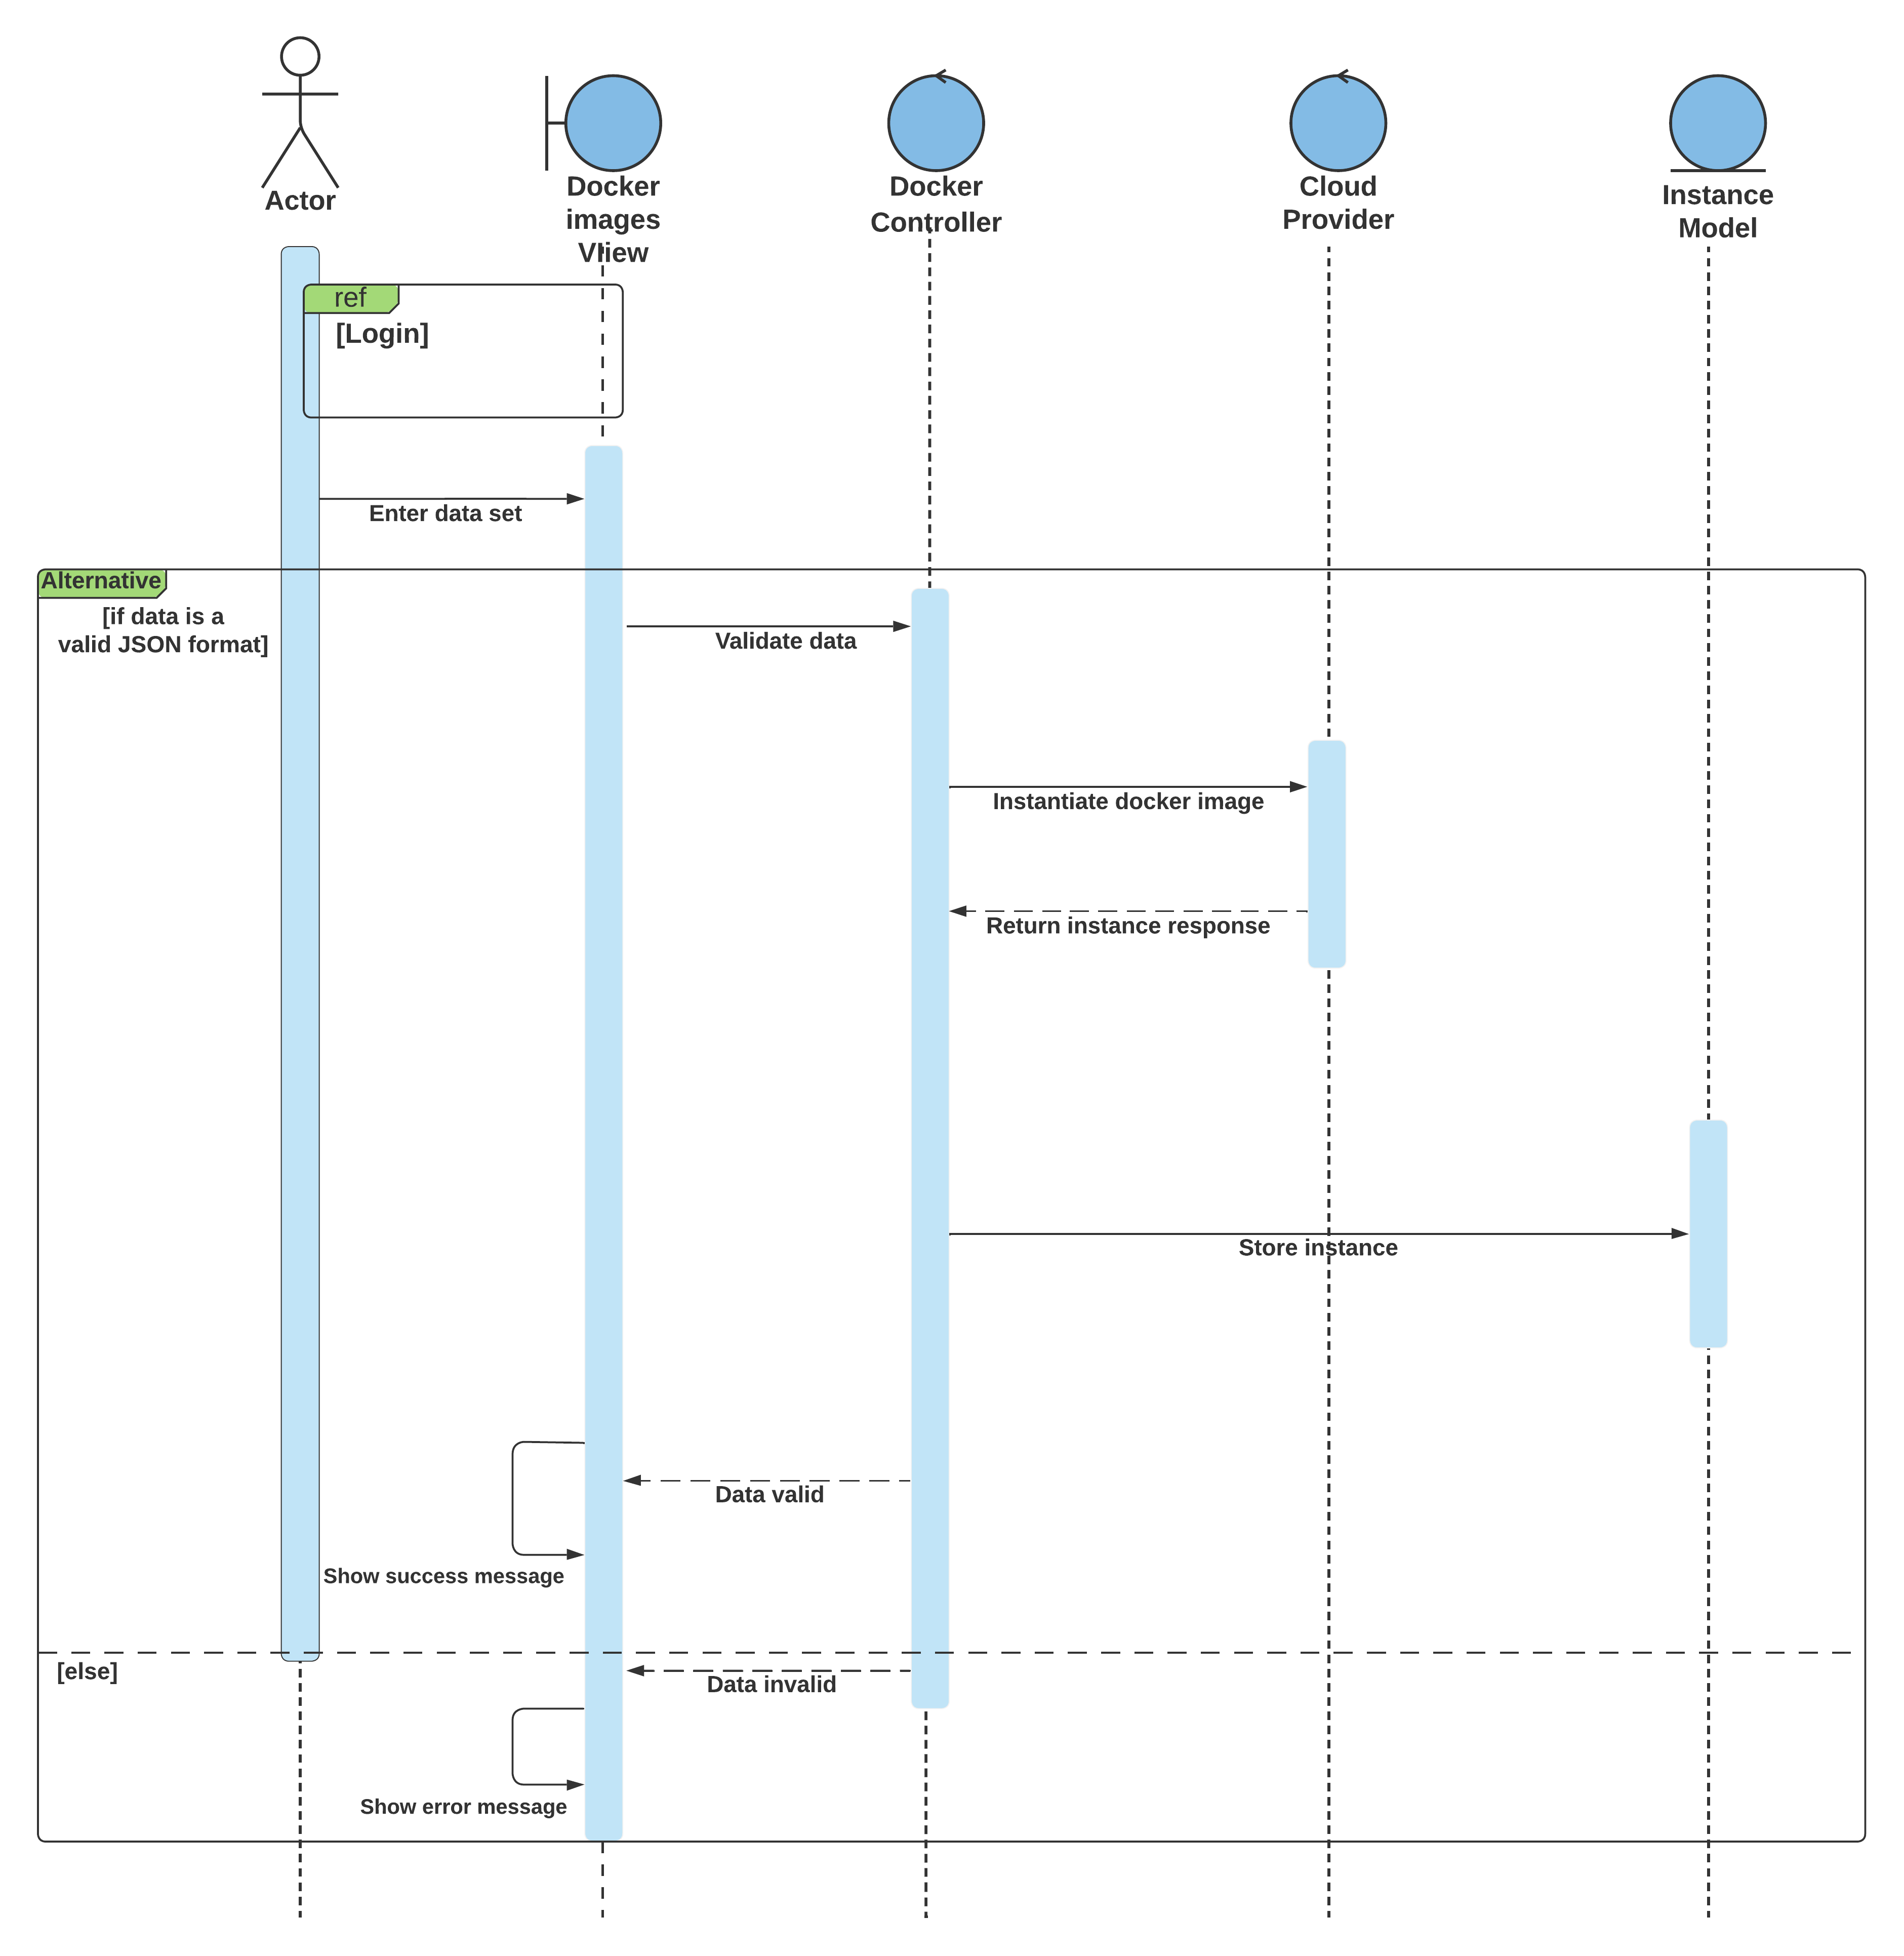
\includegraphics[width=14cm]{./chapters/sprint3/seq-instantiate.png}
  \caption{Sequence diagram: Instantiate Container}
  \label{fig:seq-instantiate}
\end{figure}

\subsection{Use case diagram of "Create Cluster"}

The following figure (\hyperref[fig:sequenece-cluster]{Figure \ref{fig:sequenece-cluster}})  represents the ``Orchestrate \ac{K8s} Cluster'' detailed use case.
\begin{figure}[h]
  \center
%\hspace*{-0.9in}
  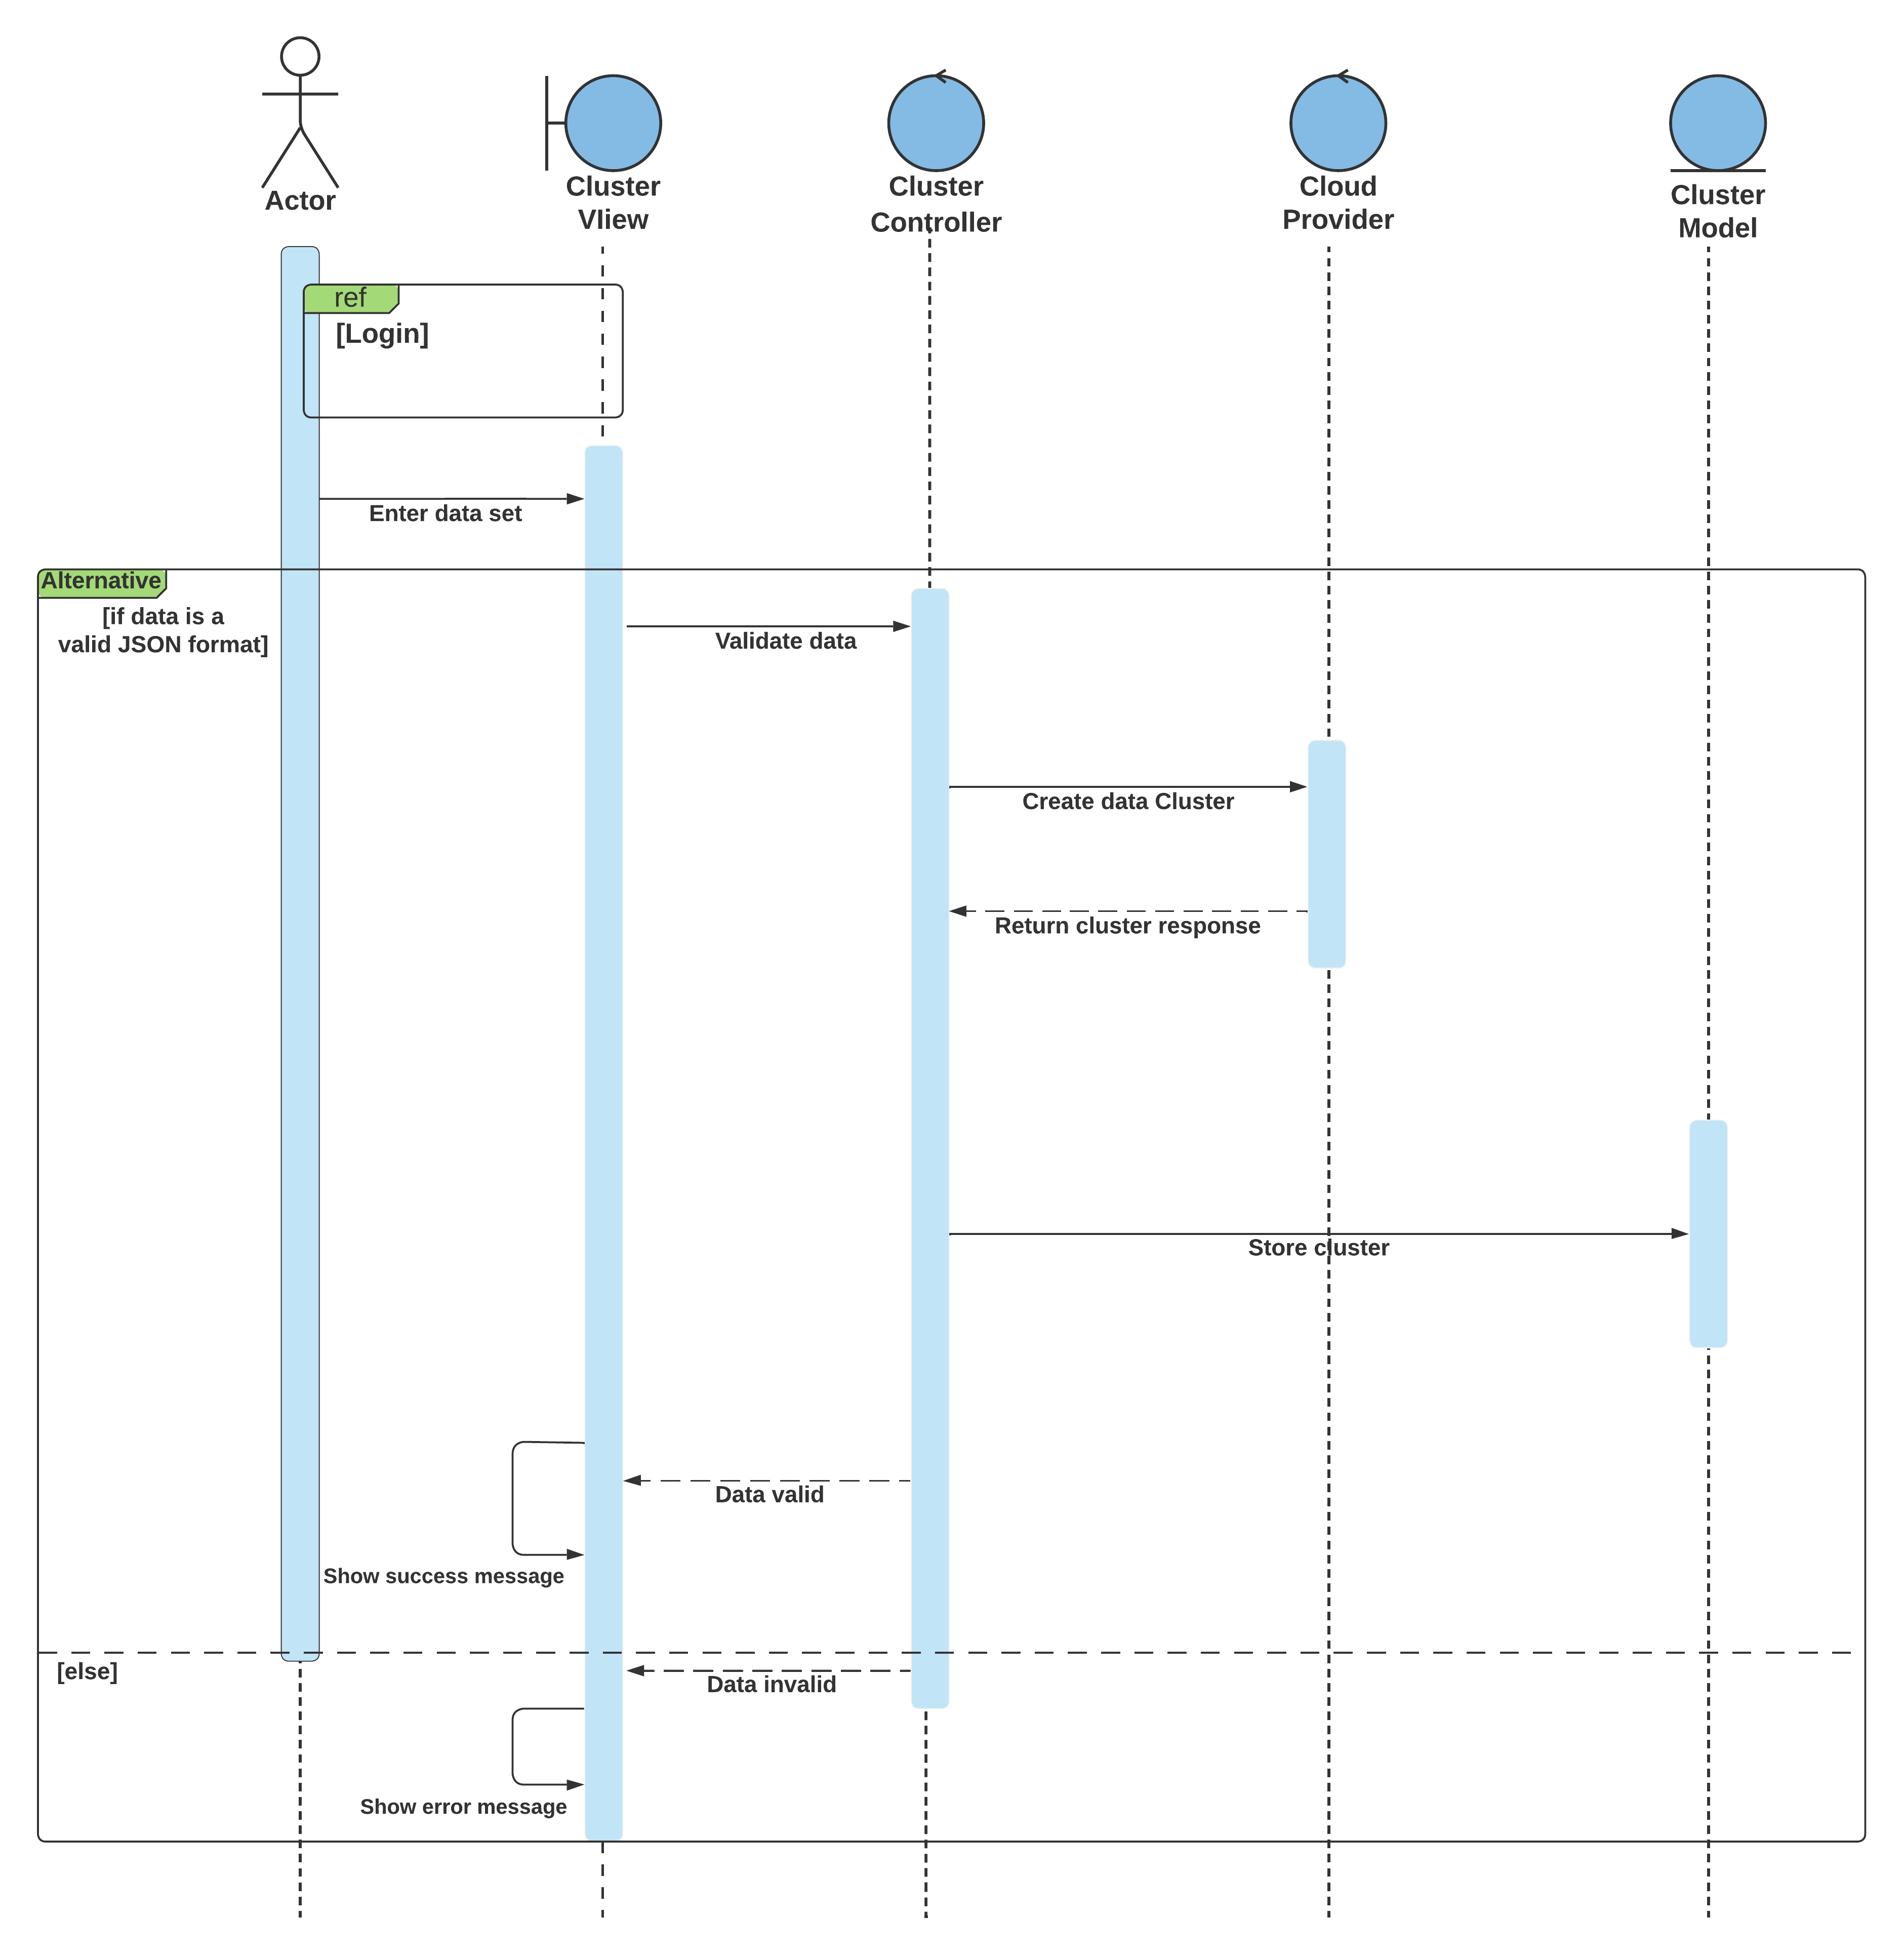
\includegraphics[width=10cm]{./chapters/sprint3/sequenece-cluster.png}
  \caption{Orchestrate K8S cluster detailed use case diagram}
  \label{fig:sequenece-cluster}
\end{figure}

\subsection{Interfaces}
In this section, we will provide screenshots and detailed explanations of the interfaces related to container management as part of Sprint 3. These interfaces cover the functionalities for fetching images, instantiating containers, and managing clusters.

The following figure (\hyperref[fig:docker-images]{Figure \ref{fig:docker-images}})  depicts the Docker images page of our application.
\begin{figure}[h]
  \center
%\hspace*{-0.9in}
  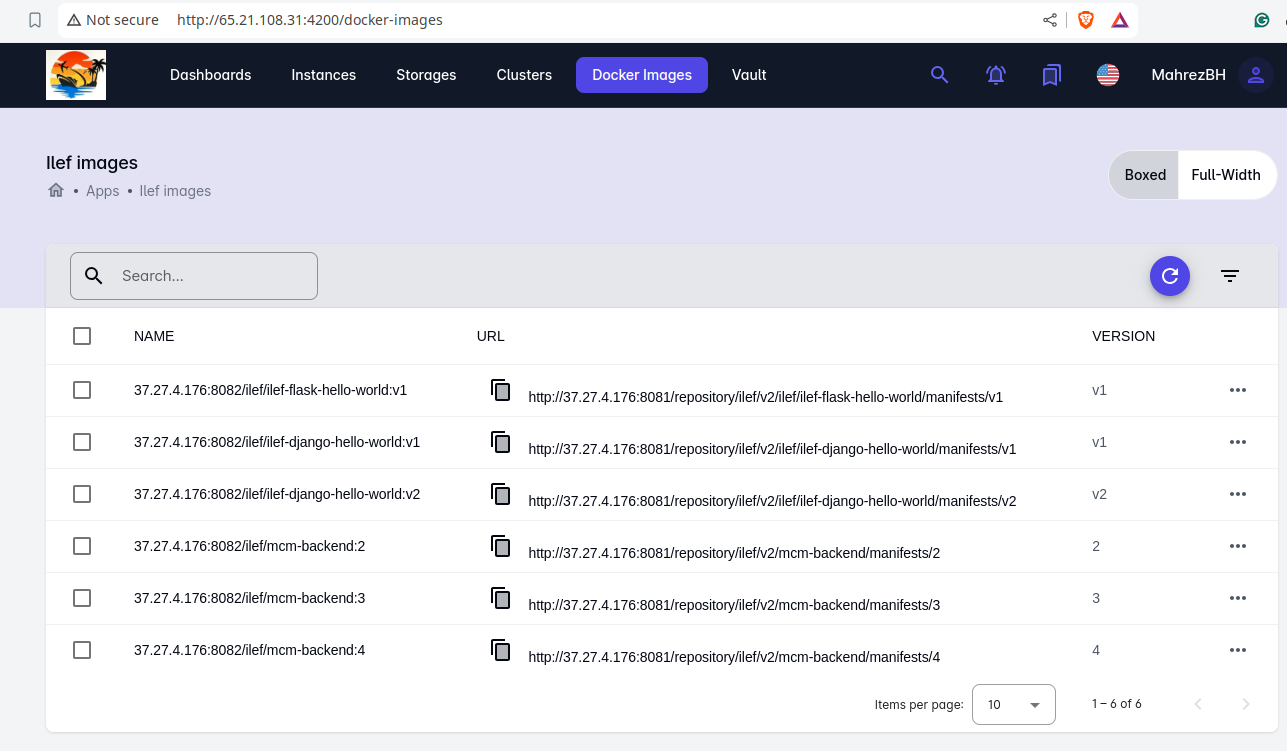
\includegraphics[width=13cm]{./chapters/sprint3/docker images.png}
  \caption{Ilef images page}
  \label{fig:docker-images}
\end{figure}

The images are fetching  from the Nexus server as the following figure  shown (\hyperref[fig:nexus-server]{Figure \ref{fig:nexus-server}}) :


\begin{figure}[h]
  \center
%\hspace*{-0.9in}
  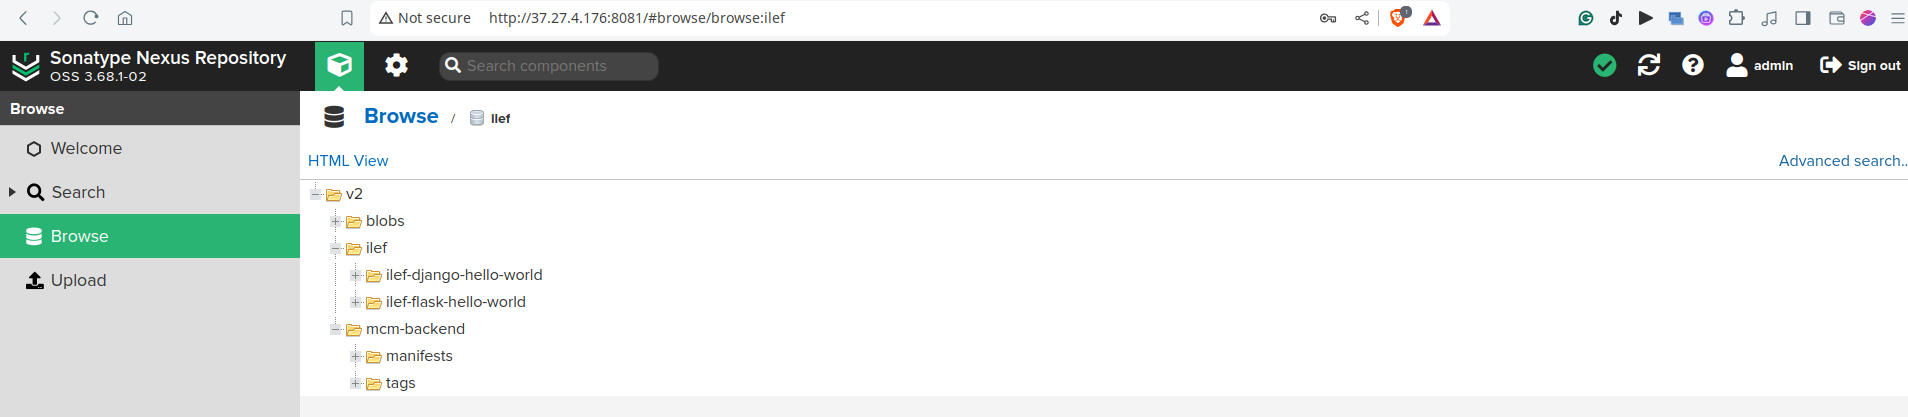
\includegraphics[width=13cm]{./chapters/sprint3/nexus.png}
  \caption{Nexus server images}
  \label{fig:nexus-server}
\end{figure}

The following figure (\hyperref[fig:clusters]{Figure \ref{fig:clusters}}) represents the Cluster page of our application.

\begin{figure}[h]
  \center
%\hspace*{-0.9in}
  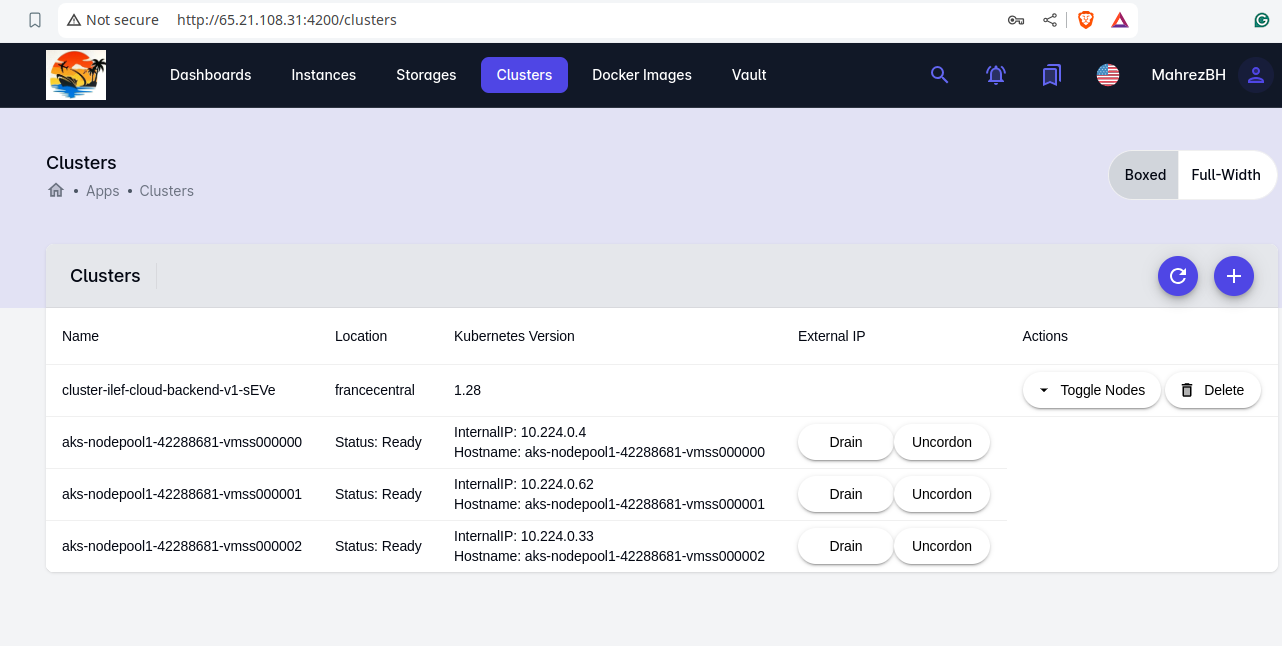
\includegraphics[width=13cm]{./chapters/sprint1/clusters.png}
  \caption{Ilef User registration page}
  \label{fig:clusters}
\end{figure}

\vspace*{7cm}

\section*{Conclusion}
In this chapter, we concentrated on Sprint 3, dedicated to container management. We developed and implemented functionalities for handling container images, including fetching images from the Nexus server, instantiating containers across various cloud providers, and managing container clusters. Use case and sequence diagrams were used to illustrate these processes clearly.


We also created intuitive interfaces to facilitate these functionalities, supporting critical operations like searching for images, creating containers, and orchestrating clusters. This has improved the overall performance and scalability of our system.


The completion of Sprint 3 has significantly enhanced our application's container management capabilities, making it more robust and adaptable to various deployment scenarios. This advancement establishes a strong foundation for future development and optimization efforts.